\saltoPag%
\section{UNIDAD 2}
    \subsection{Experimentos y teorías}
        \begin{center} \textcolor{red}{\underline{Exp. De Millikan}} \end{center}
        \indent Determinación de la masa específica del electrón.
        \begin{center} 
            \begin{tabular}{|| c | c ||}
                \hline
                \textbf{Concepto}    &   \textbf{Valores}     \\
                \hline
                \hline
                Relación carga/masa  &   $-1,76 \times 10^8 C/g$ \\
                \hline
                Carga del $e^-$      &  $-1.60 \times 10^{-19} C$ \\
                \hline
                Masa del $e^-$       &  $9,10 \times 10^{-28} g$ \\
                \hline
            \end{tabular}
        \end{center}

        \begin{center} 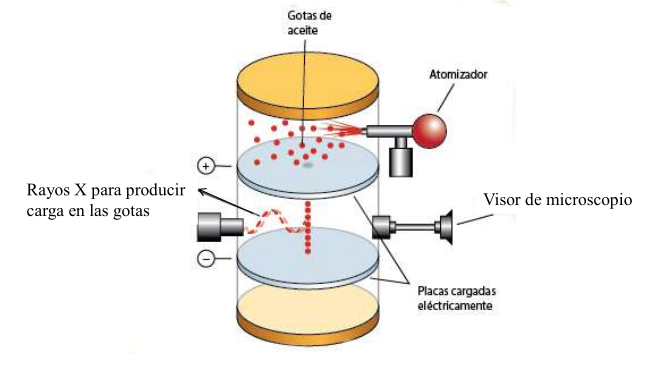
\includegraphics[width=8cm]{./imagenes/experienciaMIllikan.png} \end{center}

        \begin{center} \textcolor{red}{\underline{Radiactividad}} \end{center}
            \begin{center} 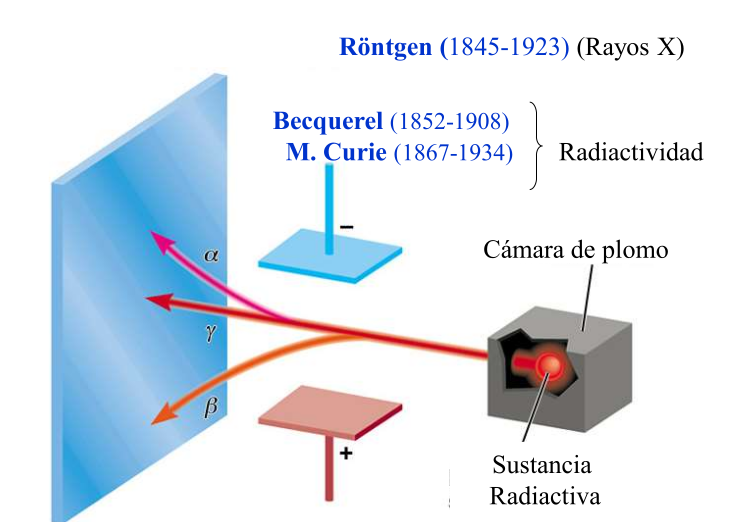
\includegraphics[width=8cm]{./imagenes/radiactividadExperimento.png} \end{center}

        \begin{center} \textcolor{red}{\underline{Modelo de Thomson}} \end{center}
        \begin{center} 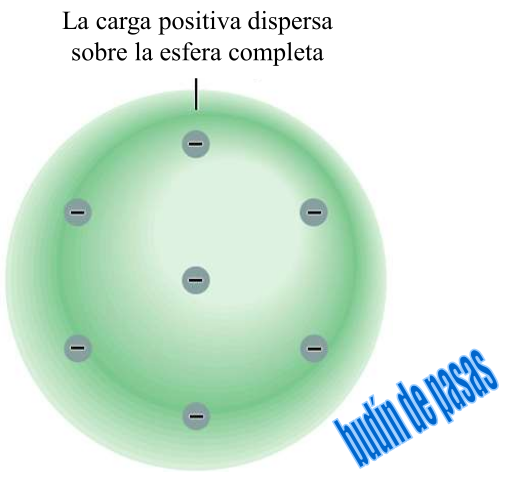
\includegraphics[width=7cm]{./imagenes/modeloDeThomson.png} \\[2cm] \end{center}
        
            \begin{center} \textcolor{red}{\underline{Exp. De Rutherford}} \end{center}
            \begin{enumerate} 
                \item La carga positiva de un átomo está concentrada en su núcleo.
                \item El protón ($p$) tiene una carga $+$, el electrón tiene carga $-$.
                \item La masa del protón es 1840 $\times$ masa del $e^-$ ($1.67 \ times 10^{-24}g$).
            \end{enumerate}

            \begin{center} 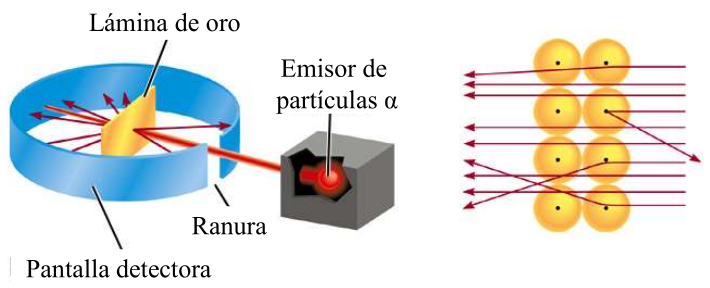
\includegraphics[width=8cm]{./imagenes/experimentoRutherford.png} \end{center}

        \begin{center} \textcolor{red}{\underline{El neutrón}} \end{center}
            \begin{center} 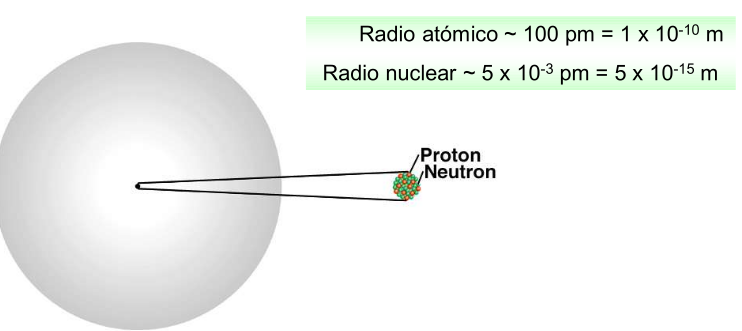
\includegraphics[width=7cm] {./imagenes/neutron.png} \end{center}

        \begin{center} \textcolor{red}{\underline{Exp. De Chadwick}} \end{center}
            \indent Se bombardeo una delgada lámina de $Be$ con partículas $\alpha$, el metal emitió una radiación de muy alta energía, similar a los rayos $\gamma$. Posteriormente se demostró que eran neutrones.

        \begin{center}
            \begin{tabular}{| c | c | c | c |}
                \hline
                \textbf{\scalebox{0.8}{Partícula}}  &
                \textbf{\scalebox{0.8}{Masa(g)}}   &
                \textbf{\scalebox{0.8}{Carga(C)}}    &
                \textbf{\scalebox{0.8}{Unidad de carga}} \\
                \hline
                \scalebox{0.8}{Electrón}            &
                \scalebox{0.8}{$9,109 \times 10^{-28}$}     &
                \scalebox{0.8}{$-1,602 \times 10^{-19}$}   & 
                \scalebox{0.8}{$-1$}    \\
                \hline
                \scalebox{0.8}{Protón} &
                \scalebox{0.8}{$1,672 \times 10^{-24}$} &
                \scalebox{0.8}{$+1,602 \times 10^{-19}$} &
                \scalebox{0.8}{$+1$} \\
                \hline
                \scalebox{0.8}{Neutrón} &
                \scalebox{0.8}{$1,674 \times 10^{-24}$} &
                \scalebox{0.8}{$0$} &
                \scalebox{0.8}{$0$} \\
                \hline
            \end{tabular}
        \end{center}

        \begin{center} \textcolor{red}{\underline{Teoría cuántica - Propiedades de las ondas}} \end{center}
            \begin{center} 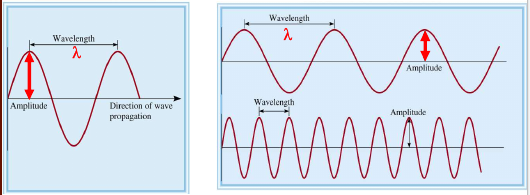
\includegraphics[width=8cm]{./imagenes/propiedadesOndas.png} \end{center}

            \begin{itemize} 
                \item \textcolor{red}{\textbf{Longitud de onda ($\lambda$):}} distancia que existe entre dos puntos idénticos en una serie de ondas.
                \item \textcolor{red}{\textbf{Amplitud:}} distancia vertical desde el punto medio de la curva hasta una cresta (punto máximo) o un valle (punto mínimo).
            \end{itemize}

        \begin{center} \textcolor{red}{\underline{Radiación electromagnética}} \end{center}
            \indent Maxwell $\Rightarrow$ \textit{''La luz está formada por ondas electromagnéticas''}.
            \saltoPag%
            \begin{center} 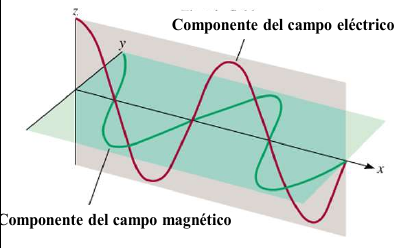
\includegraphics[width=7cm]{./imagenes/componentesDeUnaOnda.png} \end{center}
            \indent Velocidad de la luz en el vacío $\approx$ $3 \times 10^{8} m/s$.

        \begin{center} \textcolor{red}{\underline{Teoría cuántica de Planck}} \end{center}
            \indent Los sólidos cuando se calientan emiten radiación electromagnética que abarca una gama de longitudes de onda. \\
            \indent Planck definió al \textcolor{red}{\textit{cuanto}} como la mínima cantidad de energía que podía ser emitida o absorbida en forma de radiación electromagnética.

            \begin{center} \begin{tabular}{| c |} \hline \\ $E = \hbar \times v$ \\ \hline \end{tabular} \end{center}
            \indent Siendo "$\hbar$" la constante de Planck y vale $6,63 \times 10^{-34} J.s$ \\
            \indent La energía siempre se emite en múltiplos enteros y positivos de $\hbar \times v$.

    \subsection{Efecto fotoeléctrico}
        \begin{center} 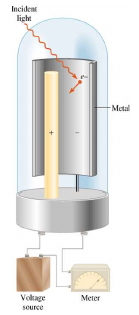
\includegraphics[width=3cm]{./imagenes/efectoFotoelectrico.png} \end{center}
        \indent La luz tiene:
        \begin{enumerate} 
            \item una naturaleza como onda electromagnética.
            \item una naturaleza como partícula (fotón).
        \end{enumerate}
        \begin{center} 
            $E = \hbar \times v$ \\
            $E = BE + KE$
        \end{center}
        \indent Siendo:
        \begin{itemize}
            \item BE\: energía de enlace.
            \item KE\: energía cinética.
        \end{itemize}
        \begin{center} \textit{Mayor frecuencia $\rightarrow$ mayor energía cinética} \end{center}
        \begin{center} \textit{Rayo de luz más intenso $\rightarrow$ mayor número de electrones emitidos.} \end{center}
        \indent La frecuencia mínima para extraer un electrón de un átomo (efecto fotoeléctrico) se denomina ''frecuencia umbral'' ($v_0$).
        \begin{center} 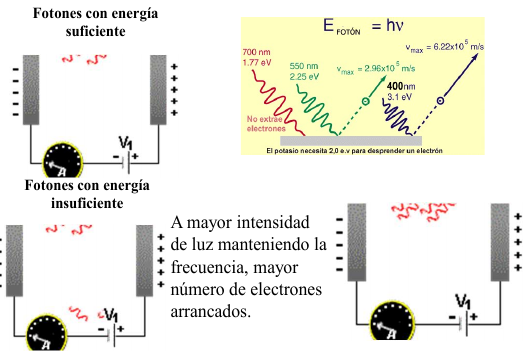
\includegraphics[width=7cm]{./imagenes/frecuenciaUmbral.png} \end{center}

    \subsection{Espectros atómicos}
        \indent Cuando a los elementos en estado gaseoso se les suministra energía (descarga eléctrica, calentamiento, etc.) éstos emiten radiaciones de determinadas longitudes de onda. \\
        \indent Estas radiaciones dispersadas en un prisma de un espectroscopio se ven como una serie de rayas, y el conjunto de las mismas es lo que se conoce como espectro de emisión. \\
        \indent Igualmente, si una luz continua atraviesa una sustancia, ésta absorbe unas determinadas radiaciones que aparecen como rayas negras en el fondo continuo (espectro de absorción). \\

    \subsection{Teoría y modelo de Bohr}
        \indent Espectro de emisión del átomo de hidrógeno.
        \begin{center} 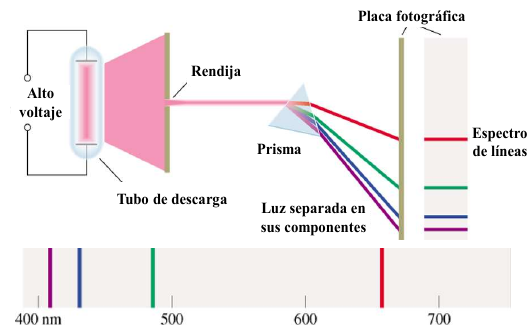
\includegraphics[width=7cm]{./imagenes/espectroEmisionHidrogeno.png} \end{center}
        
        \begin{enumerate}
            \item Los electrones se mueven en órbitas de energías específicas.
            \item Las energías del electrón están cuantiadas.
            \item Cuando existe una emisión de luz, los electrones se mueven de un nivel de energía mayor a otro menor emiten energía en forma de fotones.
            \begin{center} 
                $E_N = - R_H (\frac{1}{n^2})$
            \end{center}
        \end{enumerate}
        \saltoPag%
        \indent Siendo:
        \begin{itemize}
            \item $n$ (número cuántico principal) = 1,2,3\dots nivel energético.
            \item $R_H$ (Constante de Rydberg para el $H$) = $2,18 \times 10^{-18}J$
        \end{itemize}
        \begin{center} 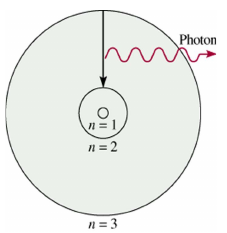
\includegraphics[width=5cm]{./imagenes/nivelesDeEnergia.png} \end{center}
        \begin{center} \textcolor{red}{\underline{Niveles de energía para el átomo de hidrógeno}} \end{center}
            \begin{center} 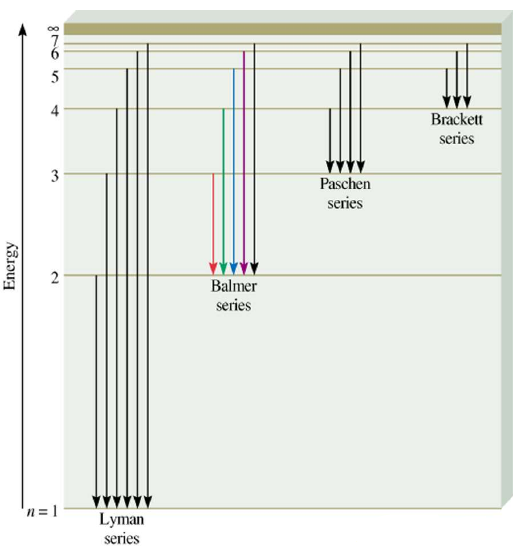
\includegraphics[width=6cm]{./imagenes/nivelesDeEnergia2.png} \end{center}

            \begin{center} 
                $E_{FOTON} = \Delta E = E_F - E_I$ \\[5pt]
                $E_F = - R_H (\frac{1}{{n_F}^{2}})$ \\[5pt]
                $E_I = -R_H (\frac{1}{{n_I}^{2}})$ \\[5pt]
                $\Delta E = R_H (\frac{1}{{n_I}^{2}} - \frac{1}{{n_F}^{2}}) = \hbar \times v$
            \end{center}
        
    \subsection{Naturaleza dual del electrón}
        \indent De Broglie razonó que si las ondas se pueden comportar como corriente de partículas (fotones), entonces la partícula como los electrones pueden tener propiedades ondulatorias. 
        \begin{center} $2 \pi r = n \lambda$ \end{center}
        \begin{center} $\lambda = \frac{\hbar}{mu}$ \end{center}        \indent Siendo:
        \begin{itemize} 
            \item $u$ = velocidad del electrón.
            \item $m$ = masa del electrón.
        \end{itemize}
    
    \subsection{Principio de incertidumbre}
        \indent Es posible conocer simultáneamente la posición y el momento $p$ ($ masa \times rapidez$) de una partícula. Así:
        \begin{center} $\Delta x \dot \Delta p \geq \frac{\hbar}{4\pi}$ \end{center}
        \indent Siento:
        \begin{itemize}
            \item $\Delta x$ = la incertidumbre en la posición.
            \item $\Delta p$ = la incertidumbre del momento de la partícula.
        \end{itemize}

    \subsection{Ecuación de onda de Schrödinger}
       \indent Schrödinger formuló una ecuación que describe el comportamiento y la energía de las partículas subatómicas. Se considera la masa ($m$) y las propiedades de onda de un electrón dada por la función de onda $\psi$.
       \begin{itemize} 
            \item El cuadrado de la función de onda ($\psi^2$) es proporcional a la probabilidad de encontrar el electrón en cierta región.
            \item La resolución matemática de la ecuación de Schrödinger para el átomo de $H$ da los tres números cuánticos que describen la distribución de los electrones en el $H$ y átomos poli-electrónicos. 
            \item Se sustituye la idea de órbita por la de orbital, como zona en donde la probabilidad de encontrar al electrón es máxima.
       \end{itemize}

    \subsection{Los números cuánticos}
        \indent Cada electrón está determinado por cuatro números cuánticos:
            \begin{itemize}
                \item \textcolor{red}{$n$}: Principal.
                \item \textcolor{red}{$l$}: Momento angular.
                \item \textcolor{red}{$m_l$}: Magnético.
                \item \textcolor{red}{$s$}: Spin.
            \end{itemize} \hfill
            
            \indent Los tres primeros determinan cada orbital, mientras que el cuarto ''$s$'' sirve para diferenciar a cada uno de los dos $e^-$ que ocupan un orbital.

        \begin{center} \textcolor{blue}{\underline{Número cuántico principal ($n$)}} \end{center}
            \begin{center} 
                \begin{tabular}{| c |}
                    \hline
                    $n = 1,2,3 \dots $ \\
                    \hline
                \end{tabular}
            \end{center} 
            \indent Distancia desde el electrón ( $e^-$ ) al núcleo.   
            \begin{center} 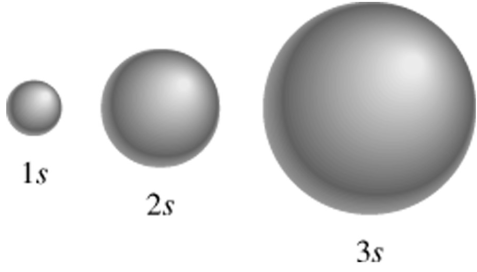
\includegraphics[width=5cm]{./imagenes/numeroCuanticoPrincipal.png} \hfill \end{center} 
            \hspace{10pt} El 90\% de los $e^-$ se encuentran en el primer orbital, a medida que se avanza en los orbitales, la probabilidad disminuye.
            \saltoPag%
            \begin{center} 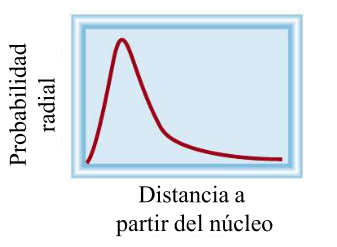
\includegraphics[width=5cm]{./imagenes/encontrarElectronOrbital.png} \end{center}

        \begin{center} \textcolor{blue}{\underline{Número cuántico de momento angular ($l$)}} \end{center}
            \begin{center} 
                \begin{tabular}{| c |}
                    \hline
                    $l$: forma de los orbitales. \\
                    \hline
                \end{tabular}
            \end{center}

            \indent Los valores de ($l$) dependen del número cuántico principal ($n$). Los valores que puede adoptar ($l$) Siento:

            \begin{center} 
                \begin{tabular}{| c |}
                    \hline
                    $l: 0,1,2 \dots n-1$ \\
                    \hline
                \end{tabular}
            \end{center}

            \begin{center} 
                \begin{tabular}{|| c | c | c ||}
                    \hline
                    \textbf{$n$} & \textbf{$l$} & \textbf{tipo de orbital} \\
                    \hline
                    \hline
                    1 & 0 & orbital s \\
                    2 & 1 & orbital p \\
                    3 & 2 & orbital d \\
                    4 & 3 & orbital f \\
                    \hline
                \end{tabular}
            \end{center}

            \indent La ecuación $(2l + 1)$ indica el número de orbitales en el subnivel. Por ejemplo, para el subnivel $p$ (momento angular $l = 1$):
            \begin{center} 
                $ 2 . 1 + 1 = 3 \rightarrow$ existen 3 orbitales $p$ ($p_x$, $p_y$, $p_z$).
            \end{center}

            \begin{center}
                \begin{tabular}{| c |}
                    \hline
                    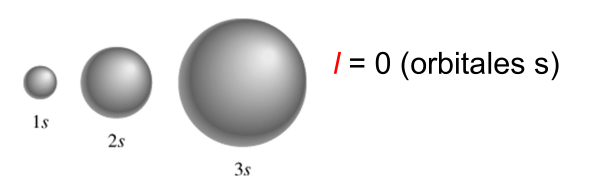
\includegraphics[width=5cm]{./imagenes/orbitalS.png}  \\
                    \hline
                    \hline
                    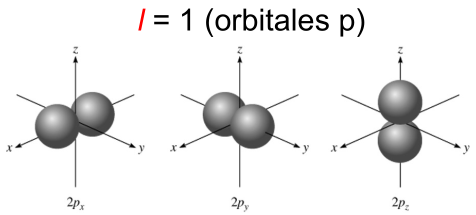
\includegraphics[width=5cm]{./imagenes/orbitalP.png} \\
                    \hline
                    \hline
                    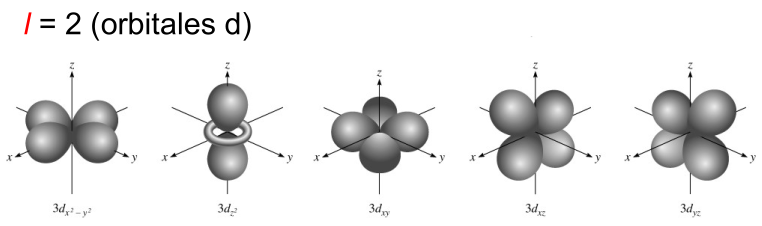
\includegraphics[width=5cm]{./imagenes/orbitalD.png} \\
                    \hline
                \end{tabular}
            \end{center}

        \begin{center} \textcolor{blue}{\underline{Número cuántico magnético ($m_l$)}} \end{center}
            \sangria Número cuántico magnético ($m_l$) describe la orientación del orbital en el espacio. Dentro de un subnivel, el valor de ($m_l$) depende del momento angular $l$.
            \begin{center} 
                \begin{tabular}{| c |}
                    \hline
                    Dado un valor de $l$ existen ($2l + 1$) valores de $m_l$: \\
                    $m_l$ = $-1, \dots, 0, \dots, +1$ \\
                    \hline
                \end{tabular} \\[10pt]
                Si $l$ = 1 (orbital $p$) $\rightarrow$ $m_l = -1, 0, +1$ \\
                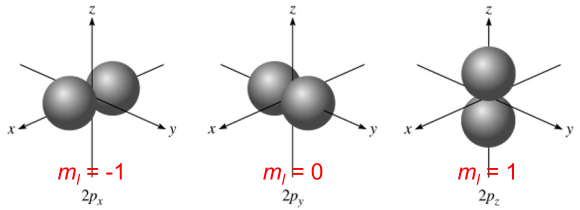
\includegraphics[width=5cm] {./imagenes/magneticoOrbitalP.png} \\
                Si $l$ = 2 (orbital $d$) $\rightarrow$ $m_l = -2, -1, 0 , +1 , +2$ \\
                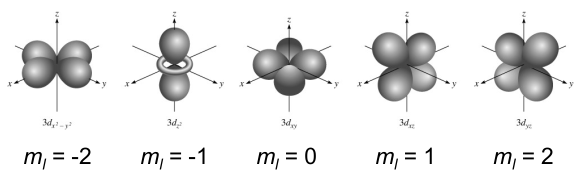
\includegraphics[width=5cm]{./imagenes/magneticoOrbitalD.png}
            \end{center}

        \begin{center} \textcolor{blue}{\underline{Número cuántico de Spin ($s$)}} \end{center}
            \begin{center} 
                \begin{tabular}{| >{\centering\arraybackslash}m{6cm} |}
                    \hline
                    Número cuántico de giro (spin)  $m_s$ \\
                    \hline
                    \hline
                    \vspace{1mm}
                    $m_s$ = $+ \frac{1}{2}$ o $- \frac{1}{2}$ \\[4pt]
                    \hline
                \end{tabular} \\[5pt]
                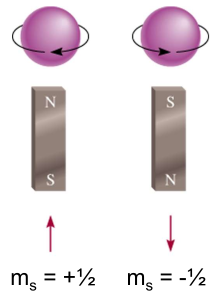
\includegraphics[width=4cm]{./imagenes/spinGiro.png} \\[10pt]

                \textbf{Resumen de los números cuánticos}
                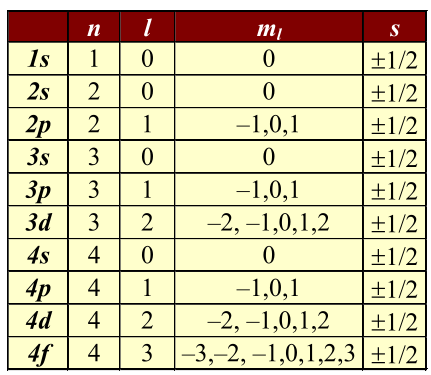
\includegraphics[width=5cm]{./imagenes/tablaNumerosCuanticos.png}
            \end{center}

    \subsection{Electrones en un diagrama de energía}
        \begin{center} \textcolor{red}{\underline{Principio de exclusión de Pauli}} \end{center}

        \indent No es posible que dos electrones tengan los mismos cuatro números cuánticos en un átomo.
        
        \begin{center} \textcolor{red}{\underline{Principio de máxima multiplicidad (regla de Hund)}} \end{center}

        \begin{itemize} 
            \item Cuando un nivel electrónico tiene varios orbitales con la misma energía, los electrones se van colocando desapareados en ese nivel electrónico.
            \item No se coloca un segundo electrón en uno de dichos orbitales hasta que todos los orbitales de dicho subnivel iso-energético están semi-ocupados.
        \end{itemize}

        \indent La energía de un electrón es proporcional al número cuántico $n$:
        \begin{center} 
            \textbf{Energía en los orbitales con un solo electrón} \\[5pt]
            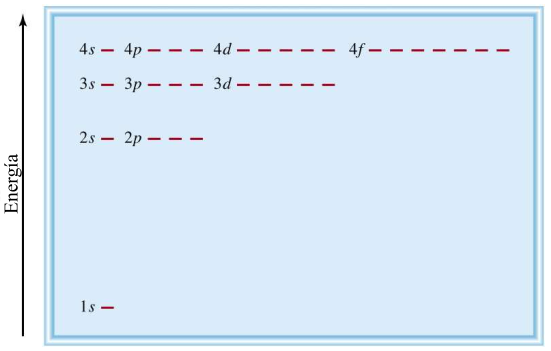
\includegraphics[width=5cm]{./imagenes/orbitalesEnergia.png}
        \end{center}

        \indent La energía del orbital que se llena primero depende de $n + l$. El número máximo de electrones por nivel ''$n$'' es igual a $2n^2$:
        \saltoPag
        \begin{center} \textbf{Energía en orbitales con varios electrones} \\[5pt] 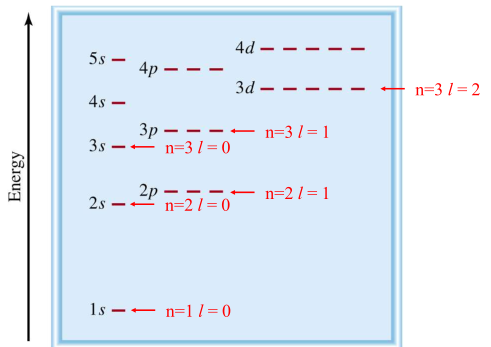
\includegraphics[width=6cm]{./imagenes/energiaOrbitalesConVariosElectrones.png} \end{center}

        \begin{center} 
            \textbf{Orden que siguen los electrones al llenar los electrones} \\[5pt]
            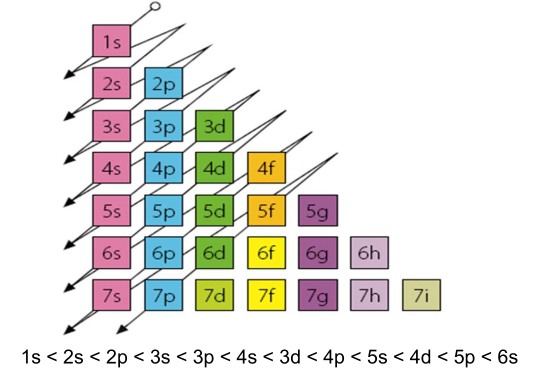
\includegraphics[width=7cm]{./imagenes/ordenQueSiguenLosElectronesAlLlenarOrbitales.png}
        \end{center}

        \indent La configuración electrónica explica cómo los electrones se distribuyen entre los diversos orbitales en un átomo.
        \begin{center} 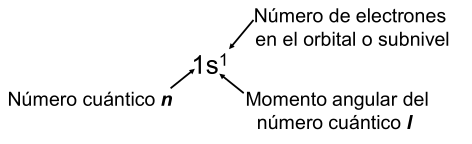
\includegraphics[width=7cm]{./imagenes/configuracionElectronica.png} \end{center}

        \begin{center} 
            \textbf{Diagrama de un orbital} \\[10pt] 
            $H$ 
            \begin{tabular}{| c |} 
                \hline 
                $\uparrow$ \\ 
                \hline 
            \end{tabular} \\[4pt] 
            \hspace{4mm} $1s^1$ 
        \end{center}

        \begin{center} \textbf{Último subnivel de energía para los elementos} \\[10pt] 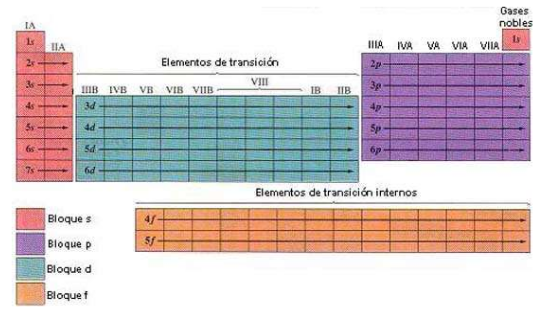
\includegraphics[width=7cm]{./imagenes/ultimoSubnivelEnergia.png} \end{center}
        \begin{center} 
            \textbf{Tipos de Spin}
            \includegraphics[width=6cm]{./imagenes/paraDiaMagnéticos.png} \\[10pt]
        \end{center}

    \subsection{La Tabla periódica}
        \indent En el siglo XIX se midieron las masas atómicas de una gran cantidad de elementos, y se observó que ciertas propiedades variaban periódicamente en relación a su masa. \\
        \indent De esa manera, hubo diversos intentos de agrupar los elementos, todos ellos usando la masa atómica como criterio de ordenación. \\
        \indent La configuración electrónica del elemento determina su posición en la tabla periódica. \\
        \indent En 1869, Mendeléyev y Meyer publicaron en forma independiente un ordenamiento de los elementos muy similar a la actual tabla periódica. \\
        \indent La clasificación de Mendeléyev es la más conocida y elaborada de todas las primeras clasificaciones periódicas. \\
        \indent Se clasificó los 63 elementos conocidos hasta entonces utilizando el criterio de masa atómica usando hasta entonces. \\
        \indent Hasta bastantes años después no se definió el concepto de número atómico puesto que no se habían descubierto los protones. \\
        \indent Dejaba espacio vacíos, que él consideró que se trataba de elementos que aún no se habían descubierto.
        \begin{center} 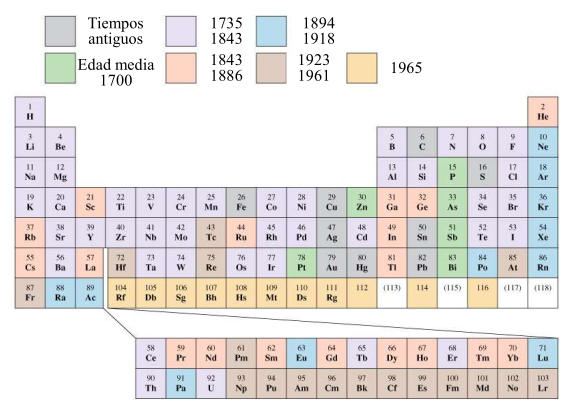
\includegraphics[width=6cm]{./imagenes/tablaPeriodicaMendeleyec.png} \end{center}
        \sangria En 1913 Moseley  ordenó los elementos de la tabla periódica usando como criterio de clasificación el número atómico. \\ 
        \indent Se enunció la ''ley periódica'': \textcolor{red}{Si los elementos se colocan según aumenta su número atómico, se observa una variación periódica de sus propiedades físicas y químicas.} 
        \saltoPag%
        \begin{center} 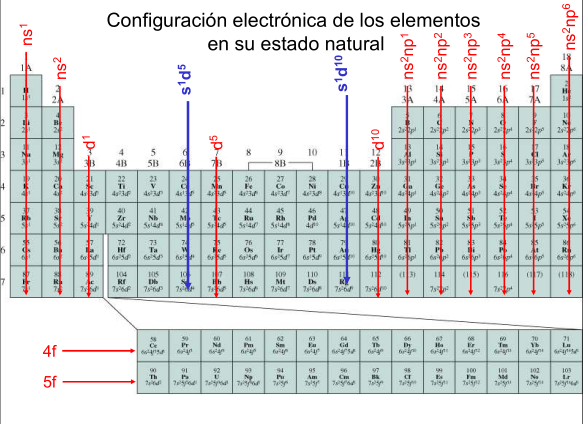
\includegraphics[width=6cm]{./imagenes/configuracionElectronicaElementosEstadoNatural.png} \end{center}
        \begin{center} \textbf{Clasificación de los elementos} \\[10pt] 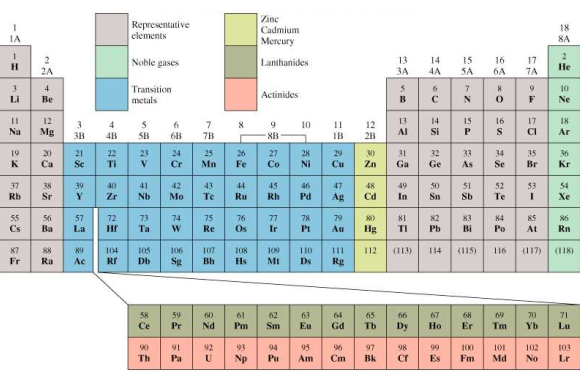
\includegraphics[width=6cm]{./imagenes/clasificacionELementos.png} \end{center}
        
    \begin{center} \textcolor{blue}{\underline{Configuraciones electrónicas de elementos}} \\ \textcolor{blue}{\underline{representativos y ubicación en la tabla}} \end{center}

        \begin{center} 
            $Na = 1s^2 2s^2 2p^6 \text{\textcolor{red}{\textbf{3}}}s^\text{\textcolor{blue}{\textbf{1}}}$ 
        \end{center}

        Siendo: 
        \begin{itemize}
            \item \textcolor{blue}{Grupo 1}
            \item \textcolor{red}{Periodo 3}
        \end{itemize}
            
        \begin{center} 
            $O = 1s^2 \text{\textcolor{red}{\textbf{2}}}s^\text{\textcolor{blue}{\textbf{2}}} \text{\textcolor{red}{\textbf{2}}}p^\text{\textcolor{blue}{\textbf{4}}}$ 
        \end{center}

        Siendo: 
        \begin{itemize}
            \item \textcolor{blue}{Grupo 6}
            \item \textcolor{red}{Periodo 2}
        \end{itemize}

        \begin{center} \textcolor{blue}{\underline{Configuraciones electrónicas de}} \\ \textcolor{blue}{\underline{cationes y aniones de}} \\ \textcolor{blue}{\underline{elementos representativos}} \end{center}
            \sangria Los átomos ceden electrones de modo que los cationes adquieren la configuración electrónica de un gas noble. 
            \begin{center} 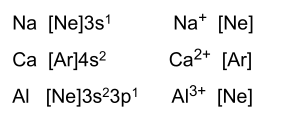
\includegraphics[width=6cm]{./imagenes/atomosCedenElectrones.png} \end{center}
            \sangria Los átomos aceptan electrones de modo que los aniones adquieren la configuración electrónica de un gas noble.
            \begin{center} 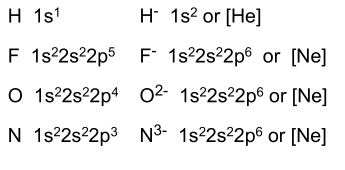
\includegraphics[width=6cm]{./imagenes/atomosAceptanElectrones.png}\end{center}

        \begin{center}
            \textbf{Aniones y cationes de los elementos representativos} \\
            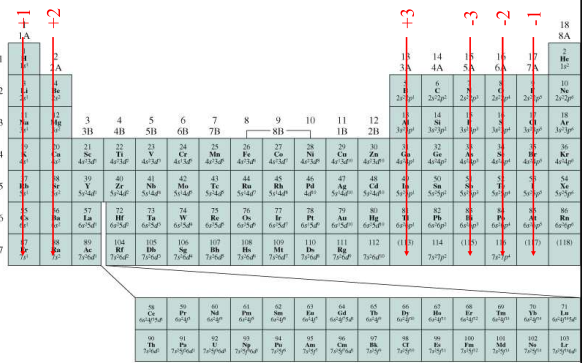
\includegraphics[width=6cm]{./imagenes/anionesYCationesDeElementosRepresentativos.png}
        \end{center}

        \begin{center} \textcolor{blue}{\underline{Carga nuclear efectiva $Z_{efectiva}$}} \end{center}
            \indent Es la ''carga positiva'' que siente un electrón.
            \begin{center}
                $Z_{efectiva} = Z - \sigma$
            \end{center}
            \indent Siendo:
            \begin{itemize}
                \item $Z$ = carga nuclear real.
                \item $\sigma$ = constante de apantallamiento.
            \end{itemize}

            \begin{center} 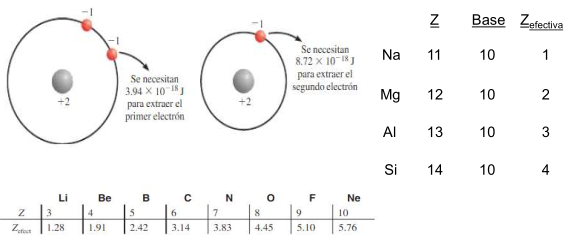
\includegraphics[width=6cm]{./imagenes/ejemplosCargaNuclearEfectiva.png} \end{center}

    \subsection{Radio atómico}
        \indent En los metales, el radio atómico es la mitad de la distancia entre dos núcleos de dos átomos adyacentes.
        \begin{center} 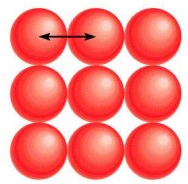
\includegraphics[width=3cm]{./imagenes/radioAtomicoMetales.png} \end{center}
        \sangria Para las moléculas di-atómicas, el radio atómico es la mitad de la distancia entre los núcleos de los dos átomos.
        \begin{center} 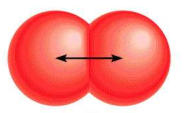
\includegraphics[width=3cm]{./imagenes/radioAtomicoDiMoleculas.png} \end{center}
        \saltoPag%
        \begin{center} \textbf{Variación de radios atómicos en tabla periódica} \\[10pt] 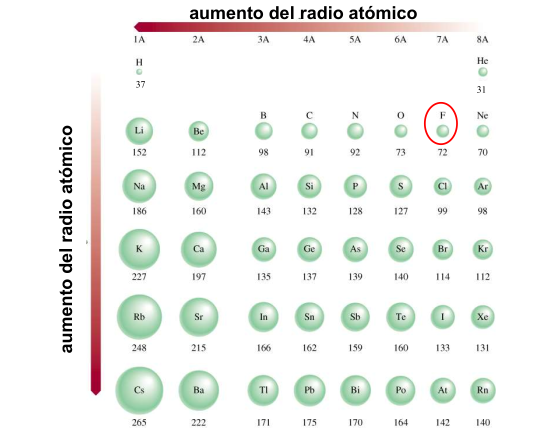
\includegraphics[width=6cm]{./imagenes/radiosAtomicosVariacion.png} \end{center}
        \begin{center} \textbf{Radio atómico v.s. Número atómico} \\[10pt] 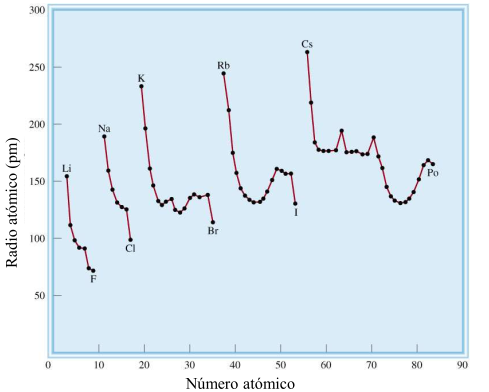
\includegraphics[width=6cm]{./imagenes/radioAtomicoVSNumeroAtomico.png} \end{center}
        \begin{center} \textbf{Radios atómicos v.s. Radios iónicos} \\[10pt] 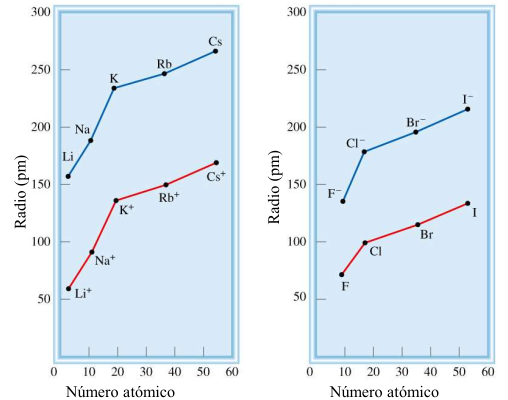
\includegraphics[width=6cm]{./imagenes/radioIonicoVSAtomico.png}  \end{center}

    \subsection{Radio iónico}
        \indent El catión siempre es más pequeño que el átomo a partir del cual se formó, mientras que el anión es más grande que el átomo a partir del cual se formó.
        \begin{center} 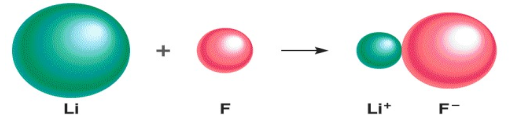
\includegraphics[width=6cm]{./imagenes/radioIonicos.png} \end{center}
        \begin{center} \textcolor{red}{\underline{Iones iso-electrónicos: comparación de radios}} \end{center}

        \indent Los iones iso-electrónicos tienen el mismo número de electrones que el gas noble más cercano. Los iones con mayor número atómico ($Z$) atraerán los $e^-$ con mayor eficacia hacia el núcleo, la nube electrónica se contrae y el radio iónico disminuye. \\
        \indent Ejemplo: Ordenar de forma decreciente el radio de los siguientes iones: 
        \begin{center} $Mg^{2+}, N^{3-}, Al^{3+}, O^{2-}, Na^{+}$ \end{center}
        \begin{center} 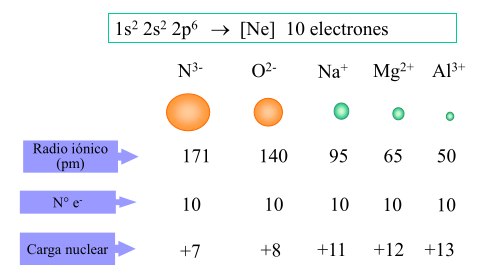
\includegraphics[width=6cm]{./imagenes/radiosIonesEjemplo.png} \end{center}

        \begin{center} \textcolor{red}{\underline{Energía de ionización}} \end{center}
            \indent Es la energía mínima necesaria para desprender un electrón de un átomo en estado gaseoso, en su estado fundamental.
            \begin{center} 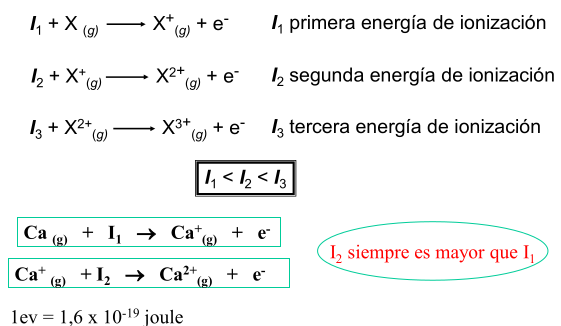
\includegraphics[width=6cm]{./imagenes/energiaDeIonizacion.png} \end{center}
            \begin{center} \textbf{Variación de la primera energía de ionización con número atómico} \\[10pt] 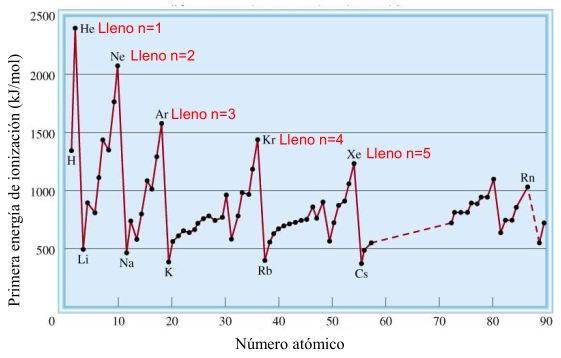
\includegraphics[width=6cm]{./imagenes/energiaDeIonizacionVSNumeroAtomico.png} \end{center}

            \begin{center} \textbf{Tendencia General en la primera energía de ionización} \\[10pt] 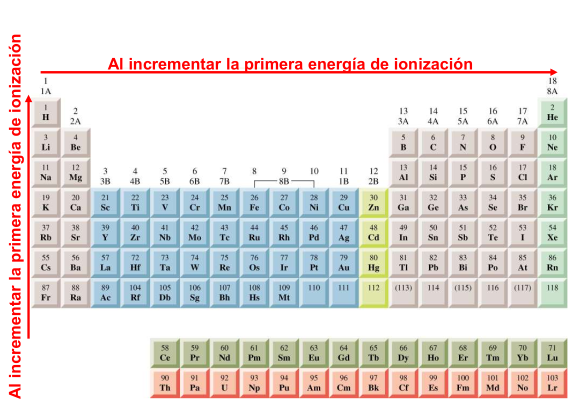
\includegraphics[width=6cm]{./imagenes/tendenciaPrimeraEnergiaDeIonizacion.png} \end{center}

        \begin{center} \textcolor{red}{\underline{Afinidad electrónica}} \end{center}
            \indent Valor negativo del cambio de energía que ocurre cuando un electrón es aceptado por un átomo en estado gaseoso para formar un anión.
            \begin{center}
                $X_{(g)} + e^- \rightarrow {X_{(g)}}^-$ \\[10pt]
                $F_{(g)} + e^- \rightarrow {F_{(g)}}^-$ $\Delta H = -326 kJ/mol$ \\
                AE = $+ 328 kJ/mol$ \\ 
            \end{center}
            \saltoPag%
            \begin{center}
                \textbf{Variación de la afinidad electrónica con el número atómico ($H - Ba$)} \\
                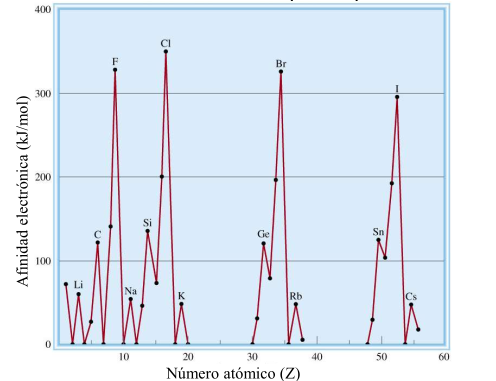
\includegraphics[width=6cm]{./imagenes/variacionAfinidadElectronicaNumeroAtomico.png}
            \end{center}

            \begin{center}
                \textbf{Irregularidades - Afinidad electrónica} \\
                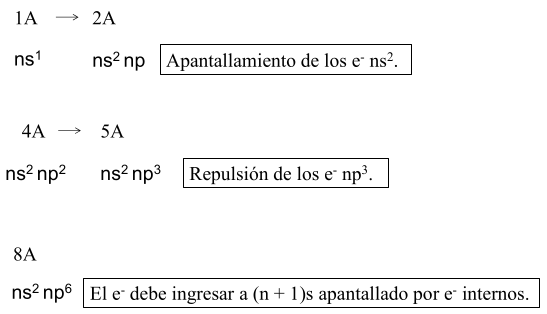
\includegraphics[width=6cm]{./imagenes/irregularidadesAfinidadElectronica.png}
            \end{center}
            

